\section{Esempio complesso}
Supponiamo di avere i dati sperimentali nella tabella \ref{tab:regrcompl} che rappresenta i tempi di caduta di un oggetto da diverse altezze:
\begin{table}[h!]
\centering
\begin{tabular}{|c|c|}
\hline
Tempo (s) & Distanza (m) \\
\hline
1.0 & 4.9 \\
2.0 & 19.6 \\
3.0 & 44.1 \\
4.0 & 78.4 \\
5.0 & 122.5 \\
\hline
\end{tabular}
\caption{Dati di un moto di caduta.}
\label{tab:regrcompl}
\end{table}



\subsection{Analisi dei Dati}
Prima di applicare il best fit lineare, calcoliamo il tempo al quadrato \( t^2 \). Infatti la formula del moto di caduta:
\[
s=\frac{1}{2}g\cdot t^2
\]
ci dice che se pongo $t^2 =t2$, la relazione tra $s$ e  $t2$ è lineare perché la formula si scrive:
\[
s=\frac{1}{2} g \cdot t2
\]
mentre quella tra $t$ ed $s$ è quadratica. A questo punto, se poniamo  $b=\frac{g}{2}$, la relazione si può scrivere:
\[
s=b\cdot t2
\]
essendo quindi una relazione senza parametro intercetta. Una volta trovato $b$, determiniamo l'accelerazione di gravità da una formula inversa.
\[
g = 2\cdot b
\]
e il suo errore propagato vale:
\[\sigma_g = 2\cdot \sigma_b
\]
essendo $\sigma_b$ l'errore sul parametro $b$ (nel codice, gli errori sulle $y$, sul parametro $a$ e sul parametro $b$ si ottengono dal vettorem
\begin{center}
\begin{tabular}{|c|c|}
\hline
Tempo (s) & Tempo al quadrato (s\(^2\)) \\
\hline
1.0 & 1.0 \\
2.0 & 4.0 \\
3.0 & 9.0 \\
4.0 & 16.0 \\
5.0 & 25.0 \\
\hline
\end{tabular}
\end{center}

Il codice Python per eseguire la regressione lineare e calcolare l'accelerazione di gravità è:

\begin{lstlisting}[caption={Calcolo della Regressione Lineare e Accelerazione di Gravità}]
import numpy as np
from scipy.optimize import curve_fit
import matplotlib.pyplot as plt

# Dati sperimentali
tempo = np.array([1.0, 2.0, 3.0, 4.0, 5.0])
distanza = np.array([4.9, 19.6, 44.1, 78.4, 122.5])
error_distanza = np.array([0.1, 0.1, 0.1, 0.1, 0.1])

# Calcolo di t^2
tempo_squared = tempo**2

# Definizione della funzione di modello lineare senza intercetta
def linear_model(t_squared, g_over_2):
    return g_over_2 * t_squared

# Regressione lineare forzata attraverso l'origine
params, covariance = curve_fit(linear_model, tempo_squared, distanza, sigma=error_distanza, absolute_sigma=True)
g_over_2 = params[0]

# Calcolo dell'accelerazione di gravità
g = 2 * g_over_2

# Calcolo dell'errore associato
std_err = np.sqrt(np.diag(covariance))
g_error = 2 * std_err[0]


print(f"Accelerazione di gravità (g): {g:.2f} +- {g_error:.2f} m/s^2")

# Creazione del grafico
plt.figure(figsize=(8, 6))
plt.errorbar(tempo_squared, distanza, yerr=error_distanza, fmt='o', label='Dati sperimentali', capsize=5)
plt.plot(tempo_squared, linear_model(tempo_squared, *params), 'r-', label='Retta di regressione')
plt.title('Misurazione dell\'Accelerazione di Gravità')
plt.xlabel('Tempo al quadrato (s^2)')
plt.ylabel('Distanza (m)')
plt.legend()
plt.grid(True)
plt.savefig('regressione2.png')
#se vuoi scaricare il file da google colab decommenta le righe:
#from google.colab import files
#files.download('regressione2.png')
plt.show()


\end{lstlisting}


Il grafico è mostrato in figura.\ref{fig:g}. L'output dello script è:
\begin{verbatim}
Accelerazione di gravità (g): 9.80 +- 0.01 m/s^2
\end{verbatim}

Segue spiegazione del codice.




\begin{figure}[!htbp] 
    \centering
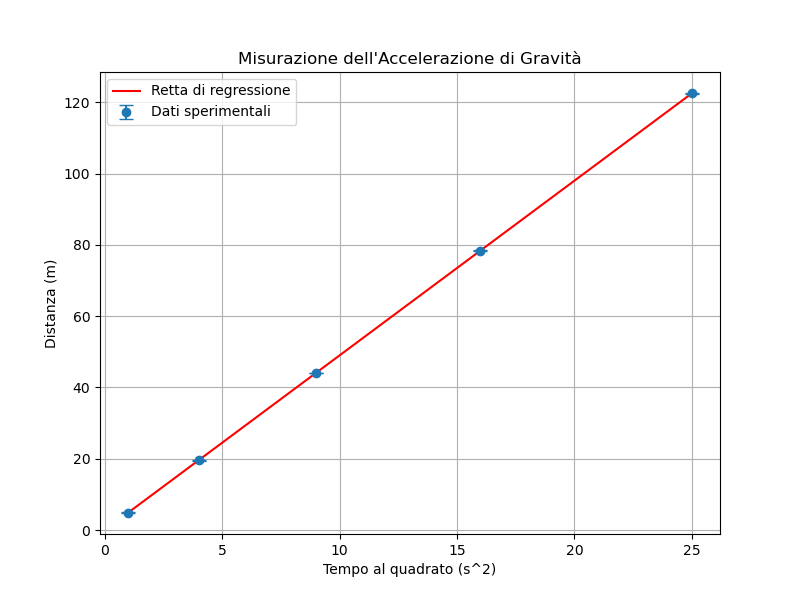
\includegraphics[scale=0.6]{g.png} 
    \caption{Grafico della regressione lineare per il calcolo dell'accelerazione dalla pendenza.}
    \label{fig:g}
\end{figure}

